\mode<all>
% Incluyo los paquetes necesarios.
% para no tener problemas con acentos etc.
\usepackage[utf8]{inputenc}
% en español
\usepackage[spanish]{babel}
%matemática
\usepackage{amsmath}
% este no se si hace falta pero por las dudas
\usepackage{graphicx}
% para incluir peliculas
\usepackage{multimedia}
% para usar segunda pantalla
\usepackage{pgfpages}
\usepackage{pgf}
% para hacer dibujitos
\usepackage{tikz}
\usetikzlibrary[automata,calc,arrows,decorations.pathmorphing,backgrounds,shapes,
patterns,positioning,fit,petri,overlay-beamer-styles]
\tikzstyle{every picture}+=[remember picture]
%recuadros sencillos
%\usepackage{tcolorbox}
% enumeradores intercambiables
\usepackage{enumerate}
% para subtitulos en figuras
\usepackage{subcaption}
%listings for code input
\usepackage{listings}
%verbatim input from file!
\usepackage{verbatim}
\usepackage{fancyvrb}
% para modificar los encabezados y pies de página.
%\usepackage{fancyhdr}
%\pagestyle{fancy}
\usepackage{standalone}

\definecolor{codegreen}{rgb}{0,0.6,0}
\definecolor{codegray}{rgb}{0.5,0.5,0.5}
\definecolor{codepurple}{rgb}{0.58,0,0.82}
%\definecolor{backcolour}{rgb}{0.95,0.95,0.0.1}

\lstset{
    basicstyle=\fontsize{8}{10}\selectfont\ttfamily, 
    backgroundcolor=\color{Beige},   
    frame=lines,
    commentstyle=\color{codegreen},
    keywordstyle=\color{magenta},
    numberstyle=\tiny\color{codegray},
    stringstyle=\color{codepurple},
    breakatwhitespace=false,         
    breaklines=true,                 
    captionpos=b,                    
    keepspaces=true,                 
    numbers=left,                    
    numbersep=5pt,                  
    showspaces=false,                
    showstringspaces=false,
    showtabs=false,                  
    tabsize=4
}



%\mode<presentation>{
% para ver las notas con la presentacion.  
%\setbeameroption{hide notes}
%para dejar las notas en la segunda patnalla
%}

% incluyo los beamercolors
%%%%%%%%%% BEAMERCOLORS
% el recuadro para el titulo
\setbeamercolor{title}{fg=white,bg=Purple}
% el recuadro para el subtitulo
\setbeamercolor{subtitle}{fg=white,bg=DarkOliveGreen}
% los títulos de las secciones tienen su colorinche:
\setbeamercolor{sectionbox}{fg=white,bg=Purple}
% cada diapositiva tendrá su color de título.
\setbeamercolor{frametitle}{fg=white,bg=ForestGreen}
% el título de las secciones tienen también su color. 
\setbeamercolor{sectiontitle}{fg=white,bg=violet}

%%%% CUSTOM BEAMERCOLORS
% estos cuadros los defino para ubicar al lector en los temas que se tratan
% son los cuadritos que aparecen arriba del título. 
\setbeamercolor{structure0}{fg=white,bg=gray}
\setbeamercolor{structure1}{fg=black,bg=DarkGray}
\setbeamercolor{structure2}{fg=black,bg=lightgray}
% defino un cuadro para usar en alguna oportunidad, creo que para titulos. 
\setbeamercolor{whitebox}{fg=black,bg=white}
% un cuadro para resaltar
\setbeamercolor{highlight1}{fg=black,bg=Gold}

% beamer colors for headers and etc.
\setbeamercolor{header1}{fg=white,bg=Blue}
\setbeamercolor{header2}{fg=black,bg=Red}
\setbeamercolor{header3}{fg=black,bg=ForestGreen}

%code block
\setbeamercolor{codeblock}{fg=Blue, bg=Beige}
\setbeamerfont{codeblock}{family=\ttfamily,size=\scriptsize}


%incluyo el tema y modificaciones
%%% BEAMER THEME
% el tema 'boxes' es igual al default pero permite definir boxes de estructura 
% a mano. 
\mode<presentation>{
  \usetheme{boxes}
  % los boxes que identifican lo que se esta leyendo
    % box de la izquierda: la materia (subtitulo)
    \addheadbox{structure2}{\quad \tiny \insertshortsubtitle}
  %  box del medio en cabecera, el titulo de la clase
    \addheadbox{structure0}{\quad \tiny  \inserttitle \quad } 
  % box en a la derecha , eltítulo de la sección. 
    \addheadbox{structure1}{\quad \tiny \insertsection}
}
% tema interno y de colores para las diapositivas normales. 
\useinnertheme{rectangles}
\usecolortheme{dove}
% la fuente de las ecuaciones
\usefonttheme[onlymath]{serif}

% entorno codeblock para meter piezas de código.
% el color se definió en BEAMERCOLORS

\newenvironment{codeblock}
{
  \begin{beamercolorbox}{codeblock}
    \usebeamerfont{codeblock}
}
{
  \end{beamercolorbox}
}



% modifico los temas
  \titlegraphic{%
\includegraphics[width=0.25\textwidth]{./PREAMBLE/logo-isabt25.png}
                
\includegraphics[width=0.25\textwidth]{./PREAMBLE/logo-isabato.png}
  		\hfill
		
\includegraphics[width=0.25\textwidth]{./PREAMBLE/ISOLOGOCNEA.png}
		\hfill
  		
\includegraphics[width=0.25\textwidth]{./PREAMBLE/unsam-horizontal.png}}

\mode<presentation>{
\setbeamertemplate{title page}[center]
{
  %
\includegraphics[width=0.25\textwidth]{./PREAMBLE/ISOLOGOCNEA.png}
  \inserttitle
  \insertsubtitle
  \insertauthor
  \insertinstitute
%  \inserttitlegraphic
}
}


% defino el template para las dapositivas con los titulos de las secciones. 
%es una recetita que saqué de algun lado. 
\setbeamertemplate{section page}{
  \begin{beamercolorbox}[ht=5ex,dp=1ex,wd=\paperwidth,center]{sectionbox}
    \begin{centering}
     \usebeamerfont{section  title} \insertsection 
    \end{centering}
  \end{beamercolorbox}
}
\AtBeginSection[]{
  \begin{frame}[plain]
    \begin{center}
    \quad \inserttitle \quad  
    \end{center}
    \sectionpage
  \end{frame}
}

% remover los simbolos de navegacion
% porque sacan espacio 
\mode<presentation>{
\setbeamertemplate{navigation symbols}{}
\setbeamertemplate{footline}[page number]
% me gustan los titulos a la derecha
\setbeamertemplate{frametitle}[default][right]%{
}
\mode<handout>{
 \setbeamertemplate{headline}{}
 \setbeamertemplate{frametitle}{}
 \setbeamertemplate{background}{
   \tikz\node [rectangle,minimum width=0.995\paperwidth,
   minimum height=0.995\paperheight,draw,anchor=south west,
   line width=2pt]  {};
 }
 \setbeamertemplate{footline}{}
}
% aparentemente el siguiente beamertemplate
%se ejecuta en modo artículo. habría que ver
%la forma de sacale probecho. 
% notar que vale solo para las framesque se incluyen 
% directamente en el artículo y no vale para 
% \includeslide.
% \setbeamertemplate{frame begin}
% \setbeamertemplate{frame end}


% no se si es el mejor lugar para definirlo, 
% pero las \includeslides deben quedar fijas al
% tamaño de la página:

%\mode<article>{
%\renewcommand\includeslide[1]{
%  \includeslide[width=\textwidth]{#1}
%}
%}

% defino el template para la diapositiva del título

%%%%%%%%%%%%%%%%%%%%%%%%%%%%%%%%
% Defino la Clase
%%%%%%%%%%%%%%%%%%%%%%%%%%%%%%%%
\subtitle[Modelización 2020]{ Modelización de Propiedades y Procesos 2021 }
\author{Ruben Weht\inst{1,2} \and Mariano Forti\inst{1,3} }
\institute{
%  \inst{1}Instituto de Tecnología Prof. Jorge Sabato
%  \and
  \inst{1}Fisica del Sólido, Edificio TANDAR, \url{weht@cnea.gov.ar},
  interno 7104
  \and
  \inst{2}División Aleaciones Especiales, Edificio 47 (microscopía),
  \url{mforti@cnea.gov.ar}, interno 7832
}

\mode<presentation>{\date{}}

\mode<article>{
  \date{
    \small
%  \textsuperscript{1} Instituto de Tecnología Prof. Jorge Sabato\\
  \textsuperscript{1}Fisica del Sólido, Edificio TANDAR, \url{weht@cnea.gov.ar},
  interno 7104 \\
  \textsuperscript{2}División Aleaciones Especiales, Edificio 47 (microscopía),
  \url{mforti@cnea.gov.ar}, interno 7832
}

%defino los encabezados y pies de págna para
% dodo el documento en función de la materia y la
% clase.
%\fancyhead[L]{\tiny Modelización de Materiales 2019}
%\fancyhead[R]{\tiny \leftmark}
}

\title{
  \mode<article>{
% 
\includegraphics[height=1cm]{./PREAMBLE/logo-isabt25.png}
    
\includegraphics[height=1cm]{./PREAMBLE/logo-isabt25.png}
\hfill

\includegraphics[height=1cm]{./PREAMBLE/ISOLOGOCNEA.png}
\hfill
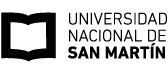
\includegraphics[height=1cm]{./PREAMBLE/logo-unsam.png}
\\} Solución de Ecuaciones Diferenciales Ordinarias }
\subject{ Métodos de Euler y de Runge-Kutta}
\keywords{Ecuaciones Diferenciales Ordinarias, Modelizacion 2020, Euler, Runge-Kutta}
% Inicia el documento.
\begin{document}

% Título de la clase. 
\mode<presentation>{
\begin{frame}[plain]
\titlepage
\end{frame}
}

\mode<article>{
\maketitle
}


\mode<all>
En este apunte no pretendemos realizar una revisión exhaustiva de los conceptos involucrados, 
simplemente debe tomarlo como una guía para implementar los métodos en un programa. Puede consultar
las teóricas para tener la descripción de los conceptos.

\section{Introducción}
\subsection{Ecuación Diferencial}

\mode<article>

Nos concentraremos en las ecuaciones diferenciales de la forma

\mode*
\begin{frame}
  \frametitle<presentation>{Ecuación Diferencial}
\begin{equation}\label{EqnEDO}
  y'- f(x, y) = 0
\end{equation}
\end{frame}
\mode<all>
\mode<article>
\noindent lo que nos dice que la derivada de la funicón depende tanto del valor de la misma función
$y$ como de la variable independiente $x$.

Para resolver esta ecuación en forma numérica, debemos discretizar la derivada, 
%
\mode*
\begin{frame}[label=FrameDiferenciasFinitas]
  \frametitle<presentation>{Método de diferencias finitas}
\begin{equation}\label{EqnDeltayDeltax}
    y' = \dfrac{y_{i+1} - y_i}{x_{i+1} - x_i} = \dfrac{y_{i+1} - y_i}{\Delta x}
\end{equation}
\end{frame}

\mode<all>
\mode<article>


\subsubsection{Problemas de condición inicial}

La \autoref{EqnDeltayDeltax}  hace evidente la naturaleza iterativa de la solución numérica. 
Necesitamos una condición inicial, es decir el valor de la función $y$ para algún valor $x_0$ 
que luego propagaremos a todos los valores posibles de $x$ con algúm método adecuado.

\mode*
\begin{frame}[label=FrameCondicionInicial]
  \frametitle<presentation>{CondicionInicial}
\begin{equation}\label{EqnCondicionInicail}
  y_0 = y(x_0)
\end{equation}
\end{frame}
\mode<all>
\mode<article>
Este tipo de razonamiento generalmente se aplica cuando la variable independiente es el tiempo, 
y la condición inicial se \emph{propaga} utilizando la \autoref{EqnDeltayDeltax}
teniendo en cuenta un \emph{paso} $\Delta x$. 
Podemos pensar que en cada paso aproximamos la función por su expansión de Taylor truncada al primer
término. 

\mode*
\begin{frame}[label=FrameIteraciones]
  \frametitle<presentation>{Naturaleza Iterativa del método}

\begin{equation}\label{EqnItera}
  \begin{aligned}
    y_1 &= y_0 + y'_0 \Delta x\\
    y_2 &= y_1 + y'_1 \Delta x\\
    \vdots \\
    y_{i+1} &= y_i + y'_i \Delta x
    \vdots \\
  \end{aligned}
\end{equation}

\end{frame}
\mode<all>
\mode<article>

Notemos que la bondad de la aproximación $y_{i+1}$ depende de la aproximación a la derivada de la 
función $y'_i$. En principio la \autoref{EqnEDO} nos da una estimación de dicha derivada, y la 
usaremos para construir nuestros métodos de solución. 

\subsection{Método de Euler}

En este método aproximamos a la función en $x_{i+1}$ por su recta tangente en $x_{i}$. 

\mode*

\begin{frame}[label=FrameMetodoEuler]
  \frametitle<presentation>{Método de Euler}
  \begin{equation}
    y_{i+1} = y_i + f(x_i, y_i ) \Delta x
  \end{equation}
\end{frame}
\mode<all>

\mode<article>

\subsection{Método de Runge-Kutta}

Para este método, se aproxima la función por su expansión de Taylor pero se
realizan correcciones sucesivas a la derivada de manera que necesitamos definir
cuatro constantes, que de penden de las anteriores, hasta poder aproximar la
derivada. 
\mode*
\begin{frame}[label=FrameMethodRungeKutta]
  \frametitle<presentation>{Método de Runge Kutta de orden 4}
\begin{equation}
  \begin{aligned}
    k_1 &= f(x_i, y_i)\\
    k_2 &= f \Big( x_i + \frac{1}{2} \Delta x, y_i + \frac{1}{2} k_1 \Delta x \Big)\\
    k_3 &= f \Big( x_i + \frac{1}{2} \Delta x, y_i + \frac{1}{2} k_2 \Delta x \Big)\\
    k_4 &= f \Big( x_i \Delta x, y_i + k_3 \Delta x \Big)\\
    y_{i+1} &= y_i+\frac{1}{6} \Big( k_1 + 2 k_2 + 2 k_3 + k_4 \Big) \Delta x
  \end{aligned}
\end{equation}
\end{frame}
\mode<all>
\mode<article>

\subsection{Ecuaciones de orden superior}

Estos métodos de propagación se aplican directamente a ecuaciones de orden 1,
puesto que dependen de aproximar la primer derivada de la función incógnita. 
Podemos extenderlo fácilmente a ecuaciones de orden superior de la siguiente manera.
Supongamos una ecuación de orden 2, 
\mode*
\begin{frame}[label=FrameEcuacionOrden2]
  \frametitle<presentation>{Ecuación de Orden dos}
  \begin{equation}
    y'' + \eta y' + f(x, y) = 0
  \end{equation}
\end{frame}
\mode<all>
\mode<article>

Vamos a operar tomando un cambio de variables sencillo para definir una nueva variable vectorial 
incógnita, 
\mode*
\begin{frame}[label=FrameVariableVectorial]
  \frametitle<presentation>{Nueva Variable Vectorial}
  \begin{equation}
    \begin{aligned}
      X &= y &\text{ (función ) } \\
      Y &= y' &\text{(derivada) }\\
      \mathbf{V} &= \begin{pmatrix} X \\ Y  \end{pmatrix} \\
	\mathbf{V'} &=  \begin{pmatrix} X \\ Y  \end{pmatrix}' &= 
	  \begin{pmatrix}   Y \\ -\eta Y - f(x, y)  \end{pmatrix}
    \end{aligned}
  \end{equation}
\end{frame}
\mode<all>
\mode<article>

Con lo cual tenemos definido una nueva ecuación vectoria, donde hemos reemplazado 
la función incógnita por un vector cuyas componentes son la función y su primera 
derivada. Hemos reemplazado también la función característica de la ecuación por una
función también vectorial, 

\mode*
\begin{frame}[label=FrameEcuacionOrdenSuparior]
  \frametitle<presentation>{Nueva Ecuacion de orden 1}
  \begin{equation}
    \mathbf{F}(x, X, Y) = \begin{pmatrix} Y\\ \eta Y - f(x, X)   \end{pmatrix}
  \end{equation}
\end{frame}
\mode<all>
\mode<article>

Resulta entonces que podemos aplicar los mismos métodos para resolver la variable
$\mathbf{V}$. Por ejemplo para el método de Euler, 
\mode*
\begin{frame}[label=FrameEulerVectorial]
  \frametitle<presentation>{Euler Vectorial}
  \begin{equation}\label{EqnEulerVec}
    \begin{aligned}
      \mathbf{V_i} &= \begin{pmatrix} X_{i-1} \\ Y_{i-1} \end{pmatrix} + 
	\Delta x F\Big( x_{i-1}, X_{i-1}, Y_{i-1} \Big) \\
	{} &= 
	\begin{pmatrix} 
	  X_{i-1} + \Delta x Y_{i-1} \\ 
	  Y_{i-1} + \Delta x \Big( \eta Y_{i-1} - f(x_{i-1} , X_{i-1}\Big)
	\end{pmatrix}
    \end{aligned}
  \end{equation}
\end{frame}
\mode<all>
\mode<article>

vemos que basta identificar la función $F(x, X, Y)$ para poder aplicar cualquiera de los métodos vistos.

\mode*

\mode<all>


\section{presentación del problema}

\subsection{Ecuación diferencial}
\section{Discretización del Problema}
\subsection{Ecuación de orden 1 en velocidad}
\subsubsection{Solución de Euler}
\subsubsection{Solución de Runge Kutta de orden 4}
\subsection{Ecuación de orden 2 en altura}

\section{Funciones}
\subsection{Método de Euler}
\subsection{Método de Runge Kutta}
\section{Soluciones}
\subsection{resolver ``a mano''}
\subsection{Resolviendo todo el probelma}
\subsection{Paso óptimo}

\newcommand\minilogo{
  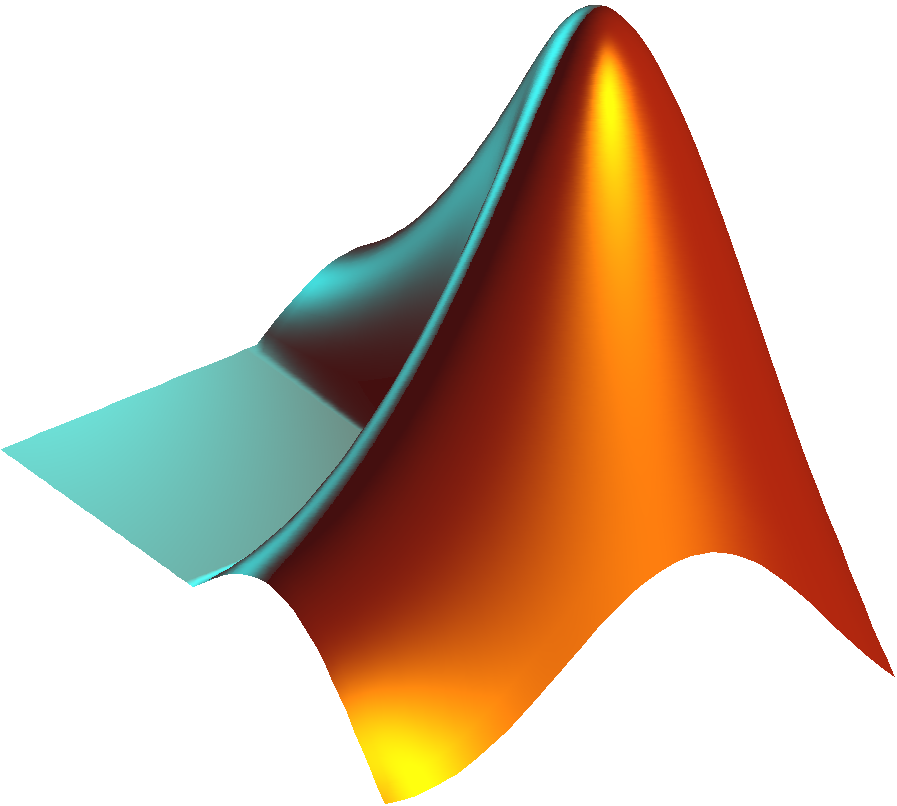
\includegraphics[width=0.5cm]{./media/Matlab_Logo.png}
}

\mode<article>{
En lo que sigue daremos una revisión
de los elementos de programación 
mínimos necesarios para esta materia.
Como lenguaje oficial elegimos 
\texttt{MATLAB}, no solo por razones
históricas, sino por su accesibilidad
para profesionales sin experiencia previa
en programación. En los casos donde sea posible, 
se darán las indicaciones equivalentes 
en otros lenguajes de uso corriente en la material 


% \begin{figure}
% \includeslide{FrameVentanaMatlab}
% \caption{Ventana de Matlab. se observan 
% el arbol de archivos del directorio
% de trabajo, el editor de guiones
% y la línea de comandos. 
% \label{FigMatlabInicio} }
% \end{figure}
}

\begin{frame}<presentation>[label=FrameMatlabPrimero]{Primeros Pasos en Matlab}
\begin{itemize}
\item[\minilogo] MATrix LABoratory
\item[\minilogo] Multiplataforma
\item[\minilogo] \url{http://www.mathworks.com/products/matlab}
\item[\minilogo] Lenguaje de programación, consola progrmable, ejecucion y redacción de scripts (guiones).
\end{itemize}
\end{frame}


\begin{frame}[label=FrameVentanaMatlab]
\frametitle<presentation>{Aspecto del Escritorio de Matlab}
%\mode<presentation>{
\begin{figure}
\begin{center}
\begin{tikzpicture}
\node [anchor=south west] (image) at (0,0) {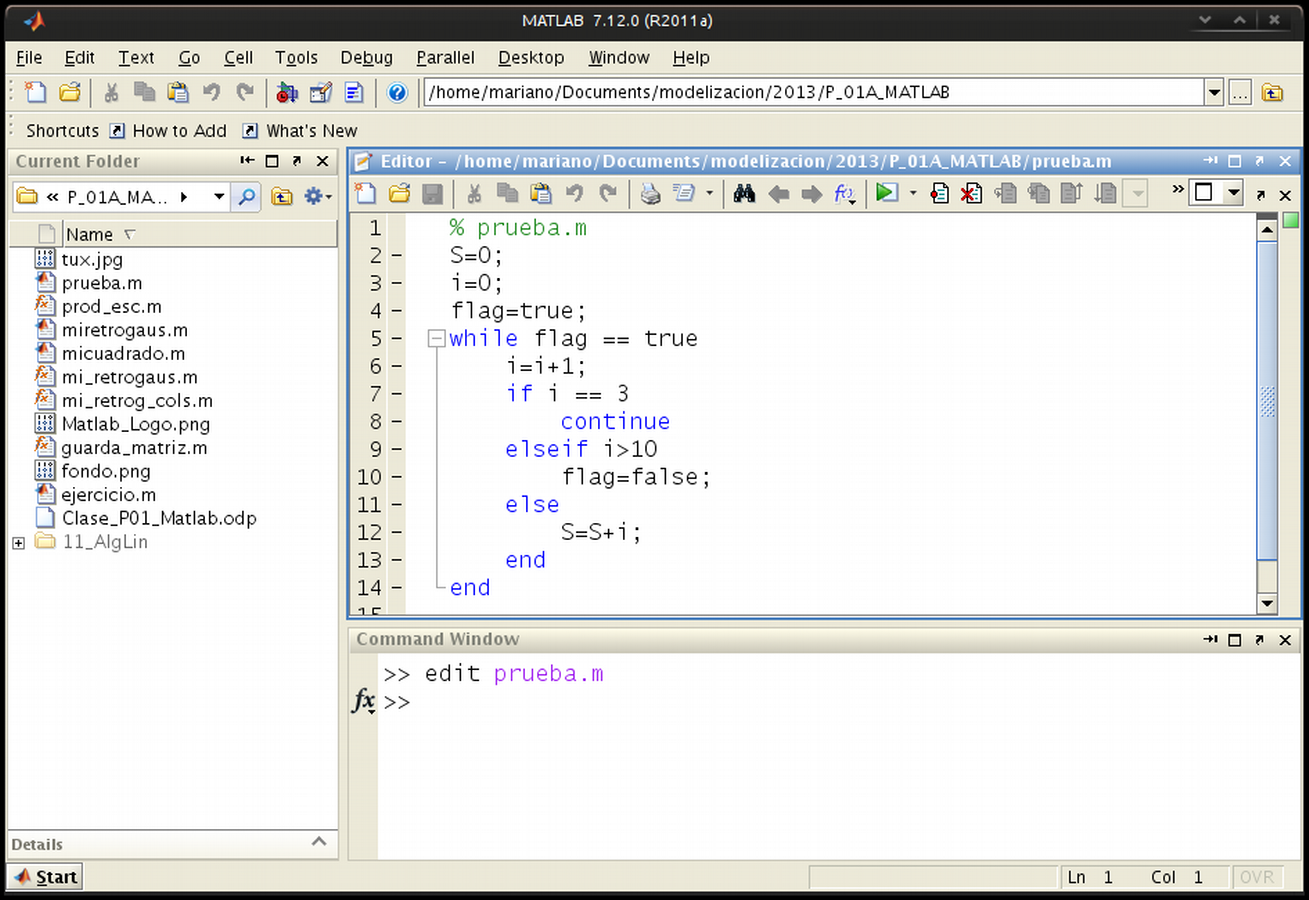
\includegraphics[width=0.7\textwidth]{./media/02-escritorio.png}};
\begin{scope}[x={(image.south east)},y={(image.north west)}]
  \node [rectangle,thick,fill=white,draw=black] at (0.15,0.2) {\small Archivos};
  \node [rectangle,thick,fill=white,draw=black] at (0.7,0.2) {\small  linea de comandos };
  \node [rectangle,thick,fill=white,draw=black] at (0.7,0.7) {\small  Editor de guiones };
\end{scope}
\end{tikzpicture}
\mode<article>{
 \caption{Ventana de Matlab. se observan 
 el arbol de archivos del directorio
 de trabajo, el editor de guiones
 y la línea de comandos. 
 \label{FigMatlabInicio}
  }
}
\end{center}
\end{figure}
%}
\mode<article>{
Busque en su pc el ícono de inicio de MATLAB, o bien inicie el programa
desde la línea de comandos. 

 Al inicar MATLAB en cualquier plataforma, se observan las ventanas de la 
 \autoref{FigMatlabInicio}. Revise las configuraciones para obtener
el escritorio que le sea cómodo. Sin embargo, puede encontrar de 
 utilidad un escritorio como el que se muestra. 

 Si bien especificamos las indicaciones para esta herramienta 
 en particular, la estructura general vale para cualquier 
 Entorno Integrado de Desarrollo (IDE) que pueda encontrar. 
} 
\end{frame}

%%\begin{frame}<presentation>[label=FrameInicioMatlab]{Escritorio y Consola de Matlab}
\begin{figure}
\subcaptionbox[.6\textwidth]{Ventana de inicio\label{FigMatlabVentanaInicio}}{
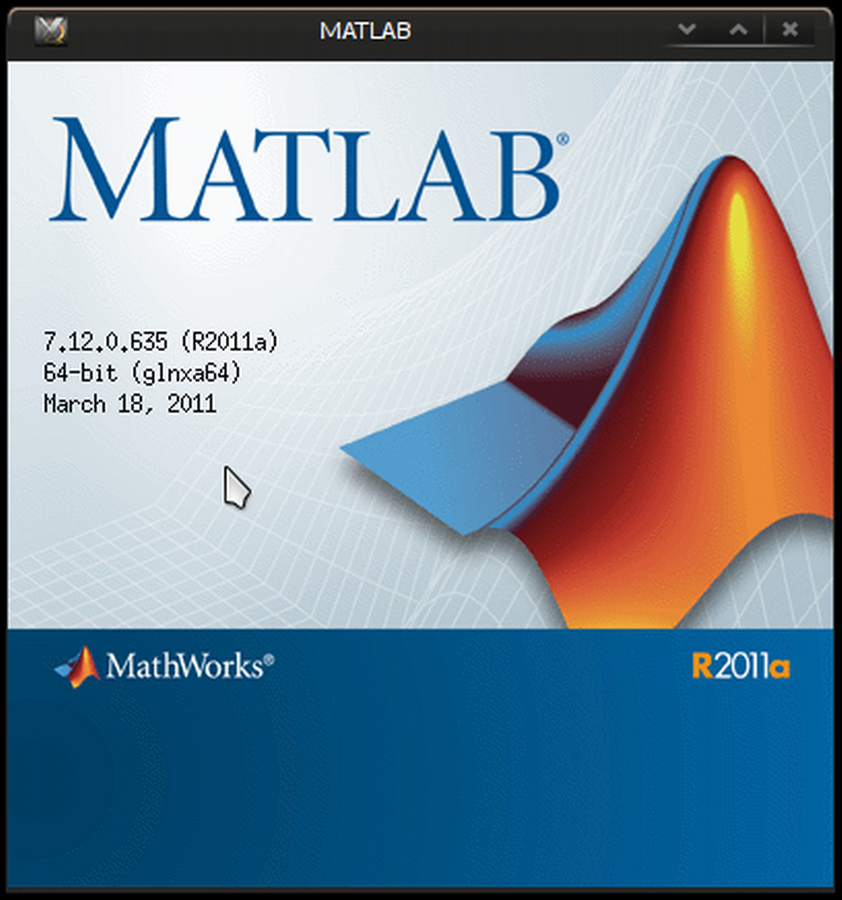
\includegraphics[width=0.2\textwidth]{./media/01-inicio.png}
}
\subcaptionbox[.4\textwidth]{Vista del Escritorio: árbol de directorio,
Editor, Ventana de comandos \label{FigMatlabEscritorio}}{
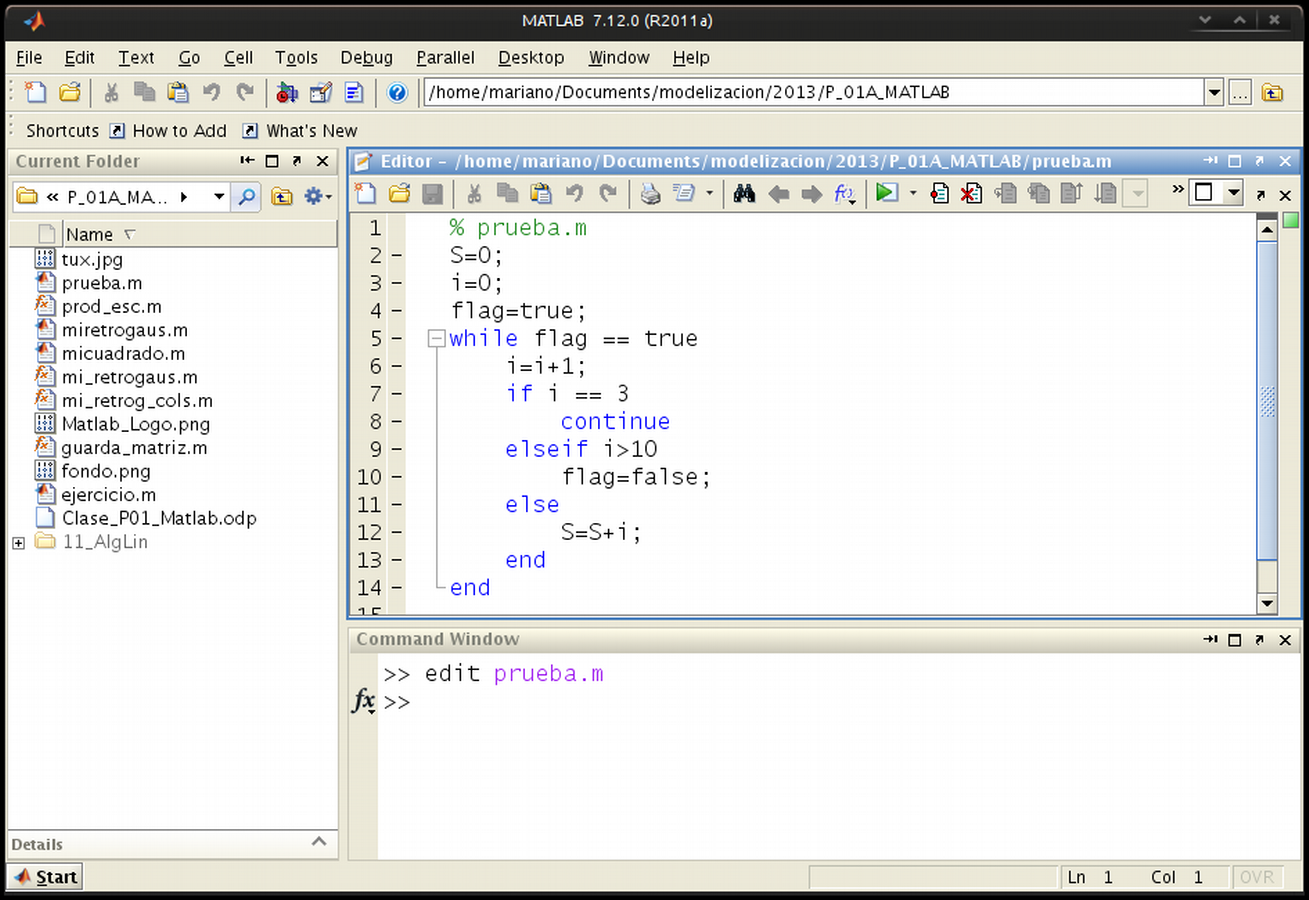
\includegraphics[width=0.4\textwidth]{./media/02-escritorio.png}
}
%\mode<article>{
%  \caption{Inicio del programa Matlab en cualquier plataforma\label{FigMatlabInicio}}
%}
\end{figure}

\end{frame}



\subsection{Asignación de Variables}

\mode*
\begin{frame}<presentation>[fragile,label=FrameAsignacionVariables]{Asignación de Variables .m}

\mode<trans>{
  Asignación de una matriz
}
\begin{columns}[T]
\column{0.5\textwidth}

 \vspace{0.5cm}

\hfill \texttt{Asignación de variables}

\vspace{1cm}

\hfill \texttt{Transponer},

\vspace{1cm}

\hfill \texttt{prompt.}

\column{0.5\textwidth}
\begin{codeblock}
  \verbatiminput{./CODEXAMPLES/ASIGNACION.m}
\end{codeblock}

\end{columns}
\end{frame}

\begin{frame}<presentation>[label=FrameAsignacionesPython]
  \frametitle{Asignacion de Variables .py}
\mode<trans>{
  Asignación de una matriz (version Python)
}
\begin{columns}[T]
\column{0.3\textwidth}

 \vspace{0.5cm}

\flushright \texttt{Asignación de variables}

\vspace{1cm}

\hfill \texttt{Transponer},

\vspace{1cm}

\hfill \texttt{prompt.}

\column{0.7\textwidth}
\begin{codeblock}
  \verbatiminput{./CODEXAMPLES/ASIGNACION.py}
\end{codeblock}

\end{columns}

\end{frame}

\mode<article>
  En cualquier lenguaje de programación, la asignación 
  de variables es la operación básica que debe aprender.
  A partir de las variables asignadas usted podrá generalizar sus
  programas para maximizar el número de casos de uso. 

  La asignación de variables se lleva a cabo mediante
  el operador \texttt{ = } de la siguente como se muestra
  en la Figura \ref{FigAsignacionVariables}. notar el uso 
  del punto y coma al final de la orden en la línea de 
  comandos. cuando no se usa, matlab muestra en pantalla
  el valor asignado a la variable.

\begin{figure}
  \includeslide[width=\textwidth]{FrameAsignacionVariables} 
\caption{Asignación y operaciones básicas en MATLAB\label{FigAsignacionVariables}}
\end{figure}

\begin{figure}
  \includeslide[width=\textwidth]{FrameAsignacionesPython} 
\caption{Asignación y operaciones básicas en Python. Observe la importación del 
        módulo \protect\emph{Numpy} para el tratamiento de Matrices. \protect\label{FigAsignacionVariablesPython}}
\end{figure}

\mode* 

\subsection{Indexación de Variables}

\begin{frame}<presentation>[fragile,label=FrameMatlabIndexacion]{Indexación de Variables}

\begin{columns}[T]
\column{0.25\textwidth}
  \vspace{0.5cm}
\hfill \texttt{Rango de filas, todas las columnas}

\column{0.25\textwidth}
  \textbf{Matlab}

\begin{codeblock}
  \verbatiminput{./CODEXAMPLES/Slice1.m}
\end{codeblock}
  \column{0.4\textwidth}
  \textbf{Python}
\begin{codeblock}
%  \verbatiminput{./CODEXAPLES/Slice1.py}
  \verbatiminput{./CODEXAMPLES/Slice1.py}
\end{codeblock}

\end{columns}
  \vspace{0.5cm}
\begin{columns}[T]
\column{0.25\textwidth}
\hfill \texttt{Vector de Índices}

\column{0.25\textwidth}
\begin{codeblock}
  \verbatiminput{./CODEXAMPLES/Slices2.m}
\end{codeblock}

  \column{0.4\textwidth}
  \begin{codeblock}
    \verbatiminput{./CODEXAMPLES/Slices2.py}
  \end{codeblock}
\end{columns}
\end{frame}

\mode<article>
Una vez asignada la matriz, es posible indexar sus componentes. 
Pueden referirse individualmente el elemento de la fila \texttt{i} y la
columna \texttt{j} pidiendo el elemento \texttt{A(i,j)}. Sin 
embargo, es posible realizar operaciones más complejas. Por ejemplo,
puede refirerse a un \emph{slice} de la matriz indicando un rango 
de índices en un vector, como se muestra en la Figura 
\ref{FigMatlabIndexacion}. La idea de los slices de arrays de una o 
más dimensiones persiste en otros lenguajes, y será particularmente
útil más adelante en esta materia, por lo que se sugiere que
verifique su implementación en el lenguaje de programación 
que elija. 

Observe en el ejemplo de la \autoref{FigMatlabIndexacion} para \emph{Python}
la necesidad de usar la función \texttt{ Numpy.ix\_ } para generar todas las 
combinaciones de índices dadas por los índices de las columnas 
\texttt{ ( i\textsubscript{1} , i \textsubscript{2} ) }
y de las columnas \texttt{ ( j\textsubscript{1} , j \textsubscript{2} ) }, 
mientras que en matlab no es necesario
una función extra. Verifique en su lenguaje de programación cómo debe indexar 
las filas y las columnas para obtener el resultado del ejeplo. 

\mode*

\begin{figure}
  \includeslide[width=\textwidth]{FrameMatlabIndexacion}
  \caption{ Indexación de Matrices con utilización de lístas de índices para
 obtener un slice de la matriz \label{FigMatlabIndexacion} }
\end{figure}

\mode*

\subsection{Sentencias de Control de Flujo: Lazos}

\begin{frame}<presentation>[label=FrameMatlabForWhile]{Control de Flujo}
\begin{columns}[T]
\column{0.5\textwidth}
\hfill \large\texttt{for}

\column{0.5\textwidth}
\begin{codeblock}
\verbatiminput{./CODEXAMPLES/suma_for.m}
\end{codeblock}
\end{columns}

\begin{columns}[T]
\column{0.5\textwidth}
\hfill \large\texttt{while}

\column{0.5\textwidth}
\begin{codeblock}
\verbatiminput{./CODEXAMPLES/suma_while.m}
\end{codeblock}

\end{columns}
\end{frame}

\mode<article>

Frecuentemente se encontrará con la necesidad de repetir una serie de 
comandos un número fintio de veces o bien hasta que se cumpla alguna 
condición lógica. Las Sentencias de Control de flujo que se usan en esas 
ocaciones son el \textbf{for} y el \textbf{while}, respectivamente, 
cuyas sintaxis se muestran en la figura \ref{FigMatlabForWhile}. A la pieza de
código que forman estas sentencias se las conoce como
lazos o bucles (loop).

\begin{figure}
  \includeslide[width=\textwidth]{FrameMatlabForWhile}
  \caption{
    Sintaxis para las sentencias for y while
  para el control de flujo de ejecución \label{FigMatlabForWhile}
}
\end{figure}

En el caso de usar la sentencia \textbf{for}, los valores que debe tomar
el iterador se dan en un rango de la forma  $[ i_{min} :  \Delta i : i_{max} ]$, 
estos valores enteros positivos. Nuevamente se ha dado la sintaxis en matlab
pero pueden encontrarse formas equivalentes en otros lenguajes. 

Luego, en el caso de utilizar la sentencia \textbf{while}, el criterio 
de ejecución se da con una sentencia lógica, por ejemplo la comparación
entre dos números reales, o simplemente la evaluación de una 
variable tipo lógico. Si se necesita un contador, en estos casos
debe actualizarse el valor del mismo en forma manual. Es buena
práctica poner además una condicón que fuerce la terminación  
del lazo en caso de que la condición lógica no se cumpla 
en una cantidad de iteraciones razonable. 

\mode*

\subsection{Control de Flujo: Condicionales}

\begin{frame}<presentation>[label=FrameMatlabIf]{Control de flujo: Condicionales} 
\begin{columns}[T]
\column{0.2\textwidth}
\hfill \large\texttt{if}

\column{0.4\textwidth}
\begin{codeblock}
\verbatiminput{./CODEXAMPLES/suma.m}
\end{codeblock}

\column{0.4\textwidth}
\begin{codeblock}
\verbatiminput{./CODEXAMPLES/suma_continue.m}
\end{codeblock}

\end{columns}
\end{frame}

\mode<article>

Otro caso de trabajo frecuente es el de tener 
la necesidad de condicionar la ejecución de 
una pieza de código a la ocurrencia de una 
condición lógica. Para esto se usa la sentencia
\textbf{if}. La estructura más general \textbf{if},
\textbf{else if}, \textbf{else} , \textbf{end} evalúa
una serie de condiciones en forma posicional  y 
excluyente, como se esquematiza en la Figura 
\ref{FigMatlabIf}. Las sentencias \textbf{else if} y 
\textbf{else} son opcionales. Si la condición 
de argunento en \textbf{if} se cumple, se ejecuta
la serie de comandos hasta \textbf{else} o 
\textbf{end}, lo que se encuentre primero. Al 
terminarse la serie de comandos, no se evalúan 
las condiciones que son argumento de los 
siguientes \textbf{else if}, sino que se
prosigue a partir de end. 

\begin{figure}
  \includeslide[width=\textwidth]{FrameMatlabIf}
  
  \caption{Esquema de la aplicación de los condicionales   para 
  evaluar piezas de código sujetas a condiciones 
  particulares o generales. Notar el uso de los comandos 
  \protect\textbf{continue} y \protect\textbf{break} para forzar la 
  omisión en un lazo o la salida del mismo
  \label{FigMatlabIf}
  }

\end{figure}

Si la condición lógica que es argumento de \textbf{if}
no se cumple, se evalúa 
la condición lógica que es argunmento del 
primer \textbf{else if}, si ésta no se cumple 
se siguen evaluendo los argumentos de las
sentencias \textbf{else if} hasta que se encuentra 
una condición verdadera. En ese caso ocurre lo 
mismo que se explicó antes: cuando se termina
de ejecutar la serie de comandos habilitados
por esta instancia de \textbf{else if}, se
prosigue a partir de \textbf{end}.

La sentencia \textbf{else} da lugar a una serie de
comandos que se ejecutarán solo si ninguna de las 
condiciones lógicas evaluadas es verdadera. 
Podría decirse que marca lo que debe ejecutarse por 
descarte de las condiciones evaluadas. 

En forma general, puede tenerse en cuenta que las 
condiciones sobre las sentencias \textbf{if}, 
\textbf{else if} \emph{ detectan} casos especiales
mientras que \textbf{else} da lugar a la ejecución
sobre el caso más general pero en forma 
excluyente de los casos particulares. Este 
concepto nos será de utilidad en la separación
de las condiciones de contorno sobre un 
recinto de integración para la solución
de ecuaciones diferenciales. 

\mode*

\subsection{Operadores básicos}

\mode<article>

Cualquier lenguaje de programación con orientación a cálculo numérico soporta 
las operaciones artiméticas básicas \texttt{+}, \texttt{-}, \texttt{/} (división) 
y \texttt{*} (multiplicación).
No pretendemos aquí dar una lista exhaustiva
de todas ellas pero puede consultar las tablas al final 
de este apunte para consultas.

Quizá sea útil a esta altura hacer alguna diferencia entre las operaciones 
aritméticas y las operaciones \emph{elemento a elemento}. Por ejemplo en \texttt{Matlab}
para operar los elementos de matrices elemento a elemento puede usar los operadores 
básicos precesidos por un punto (\texttt{.}), mientras que los operadores 
comunes se utilizan como operaciones matriciales. En otros lenguages como Python 
las operaciones aritméticas implican operar por elemento y para realizar operaciones 
matriciales debe recurrir a funciones especiales como \texttt{matmul} (para 
multiplicacion matricial).

\begin{figure}

  \includeslide[width=\textwidth]{FrameOperators}

\end{figure}

\mode*

\begin{frame}<presentation>[label=FrameOperators]
  \frametitle{Operadores Básicos}
  \begin{columns}
    \column{0.5\textwidth}

    \texttt{Operaciones entre matrices}

    \flushright
      \rowcolors{1}{Green!70}{green!70}
      \begin{tabular}{ l c } 
	suma & \texttt{+}  \\
	resta & \texttt{-}  \\
	multiplicacion & \texttt{*} \\
	división & \texttt{/} \\
	exponente & \texttt{\^} \\
	menor & \texttt{<}  \\
	mayor & \texttt{>}   \\
	menor o igual & \texttt{<=} \\
	mayor o igual & \texttt{>=} \\
	distinto & \texttt{\textasciitilde{}= }
      \end{tabular}

    \column{0.5\textwidth}

    \begin{codeblock}
      \verbatiminput{CODEXAMPLES/BasicOperators.m}
    \end{codeblock}

  \end{columns}
\end{frame}

\mode<all>

\subsubsection{Operadores comparativos}

\mode<article>

Los operadores de comparación básicos también son soportados en 
programación los símbolos típicos, \texttt{>}, \texttt{<}, \texttt{==},
\texttt{<=}, \texttt{>=} con significado obvio, mientras que el 
operador distinto puede tener distintas sintaxis, por ejemplo \texttt{\textasciitilde{}=}
en \texttt{Matlab} o \texttt{!=} en \texttt{Python}. 

Los operadores comparativos serán importantes para la evaluación 
de condiciones que por ejemplo condionen la ejecución de alguna instrucción.
Se verán ejemplos de uso al introducir los condicionales.


\subsubsection{Operadores Lógicos}


Los operadores lógicos son útiles para conjugar o combinar varias sentencias de 
comparación a la hora de condicionar la ejecución de un segmento de código. 
Típicamente las sentencias \texttt{\&}(and), \texttt{|} (or), y la negación \texttt{!} en matlab 
o \texttt{not} en python se utilizan para su funcion obvia, pero tamvién estan sus 
valores excluyentes. Su uso quedará aclarado al introducir las sentencias de control de flujo.
Para un uso avanzado de los operadores lógicos le aconsejamos investigar y consultar
sobre las reglas de \texttt{De Morgan} y las tablas de verdad.

En genral también encontrará disponibles las variables lógicas \texttt{verdadero} y 
\texttt{falso}, en \texttt{Matlab} \texttt{true}, \texttt{false} o en python 
\texttt{True}, \texttt{False}. Con ellas podrá incluso generar vectores que 
muchas veces serán útiles según la aplicación.

\mode*

\mode<all>

\subsection{Sentencias de Control de Flujo: Lazos}

\mode<article>

Frecuentemente se encontrará con la necesidad de repetir una serie de 
comandos un número fintio de veces o bien hasta que se cumpla alguna 
condición lógica. Las Sentencias de Control de flujo que se usan en esas 
ocaciones son el \textbf{for} y el \textbf{while}, respectivamente, 
cuyas sintaxis se muestran en la \autoref{FigMatlabForWhile}. A la pieza de
código que forman estas sentencias se las conoce como
lazos o bucles (loop).

\begin{figure}
  \includeslide[width=\textwidth]{FrameMatlabForWhile}
  \caption{
    Sintaxis para las sentencias for y while
  para el control de flujo de ejecución \label{FigMatlabForWhile}
}
\end{figure}

En el caso de usar la sentencia \textbf{for}, los valores que debe tomar
el iterador se dan en un rango de la forma  $[ i_{min} :  \Delta i : i_{max} ]$, 
estos valores enteros positivos. Nuevamente se ha dado la sintaxis en matlab
pero pueden encontrarse formas equivalentes en otros lenguajes. 

Luego, en el caso de utilizar la sentencia \textbf{while}, el criterio 
de ejecución se da con una sentencia lógica, por ejemplo la comparación
entre dos números reales, o simplemente la evaluación de una 
variable tipo lógico. Si se necesita un contador, en estos casos
debe actualizarse el valor del mismo en forma manual. Es buena
práctica poner además una condicón que fuerce la terminación  
del lazo en caso de que la condición lógica no se cumpla 
en una cantidad de iteraciones razonable. 

\mode*

\begin{frame}<presentation>[label=FrameMatlabForWhile]{Control de Flujo}
  \begin{columns}
    \column{0.2\textwidth}
    \hfill

    \column{0.4\textwidth}
    \center{ \textbf{Matlab} }

    \column{0.4\textwidth}
    \center{\textbf{Python}}
  \end{columns}

  \begin{columns}[T]
    \column{0.2\textwidth}
      \flushright \large\texttt{for}

    \column{0.4\textwidth}
      \begin{codeblock}
	\verbatiminput{./CODEXAMPLES/suma_for.m}
      \end{codeblock}

    \column{0.4\textwidth}
      \begin{codeblock}
	\verbatiminput{./CODEXAMPLES/suma_for.py}

      \end{codeblock}

  \end{columns}

  \begin{columns}[T]
    \column{0.2\textwidth}
    \flushright \large\texttt{while}

    \column{0.4\textwidth}
      \begin{codeblock}
	\verbatiminput{./CODEXAMPLES/suma_while.m}
      \end{codeblock}

    \column{0.4\textwidth}
      \begin{codeblock}
	\verbatiminput{./CODEXAMPLES/suma_while.py}
      \end{codeblock}

  \end{columns}
\end{frame}

\mode<all>


\subsection{Control de Flujo: Condicionales}

\mode<article>

Otro caso de trabajo frecuente es el de tener 
la necesidad de condicionar la ejecución de 
una pieza de código a la ocurrencia de una 
condición lógica. Para esto se usa la sentencia
\textbf{if}. La estructura más general \textbf{if},
\textbf{else if}, \textbf{else} , \textbf{end} evalúa
una serie de condiciones en forma posicional  y 
excluyente, como se esquematiza en la 
\autoref{FigMatlabIf}. Las sentencias \textbf{else if} y 
\textbf{else} son opcionales. Si la condición 
de argunento en \textbf{if} se cumple, se ejecuta
la serie de comandos hasta \textbf{else} o 
\textbf{end}, lo que se encuentre primero. Al 
terminarse la serie de comandos, no se evalúan 
las condiciones que son argumento de los 
siguientes \textbf{else if}, sino que se
prosigue a partir de end. 

\begin{figure}
  \includeslide[width=\textwidth]{FrameMatlabIf}
  
  \caption{Esquema de la aplicación de los condicionales   para 
  evaluar piezas de código sujetas a condiciones 
  particulares o generales. Notar el uso de los comandos 
  \protect\textbf{continue} y \protect\textbf{break} para forzar la 
  omisión en un lazo o la salida del mismo
  \label{FigMatlabIf}
  }

\end{figure}

Si la condición lógica que es argumento de \textbf{if}
no se cumple, se evalúa 
la condición lógica que es argunmento del 
primer \textbf{else if}, si ésta no se cumple 
se siguen evaluendo los argumentos de las
sentencias \textbf{else if} hasta que se encuentra 
una condición verdadera. En ese caso ocurre lo 
mismo que se explicó antes: cuando se termina
de ejecutar la serie de comandos habilitados
por esta instancia de \textbf{else if}, se
prosigue a partir de \textbf{end}.

La sentencia \textbf{else} da lugar a una serie de
comandos que se ejecutarán solo si ninguna de las 
condiciones lógicas evaluadas es verdadera. 
Podría decirse que marca lo que debe ejecutarse por 
descarte de las condiciones evaluadas. 

En forma general, puede tenerse en cuenta que las 
condiciones sobre las sentencias \textbf{if}, 
\textbf{else if} \emph{ detectan} casos especiales
mientras que \textbf{else} da lugar a la ejecución
sobre el caso más general pero en forma 
excluyente de los casos particulares. Este 
concepto nos será de utilidad en la separación
de las condiciones de contorno sobre un 
recinto de integración para la solución
de ecuaciones diferenciales. 


\mode*

\begin{frame}<presentation>[label=FrameMatlabIf]{Control de flujo: Condicionales} 
\begin{columns}[T]
\column{0.2\textwidth}
\hfill \large\texttt{if}

\column{0.4\textwidth}
\begin{codeblock}
\verbatiminput{./CODEXAMPLES/suma.m}
\end{codeblock}

\column{0.4\textwidth}
\begin{codeblock}
\verbatiminput{./CODEXAMPLES/suma_continue.m}
\end{codeblock}

\end{columns}
\end{frame}

\mode<article>

En la utilización de las distintas herramientas de control de flujo conviene tener a mano
las tablas de verdad. Estas constituyen una serie de operaciones lógicas que pueden servir
para combinar condiciones de ejecución.

\begin{frame}<presentation>[label=FrameTablaVerdad]
  \frametitle{Tabla de verdad:}

\end{frame}
\mode<all>

\mode<all>
\subsection{Entrada y Salida de datos}

\mode<article>

El registro de los resultados de un problema es tan 
importante como la trazabilidad de los datos 
que se tuvieron en cuenta para resolverlo. Por lo tanto, 
en general se guardan ambos tipos de datos en archivos, 
que serán escritos y leídos por nuestra herramienta 
informática oportunamente. notar entonces que la legibilidad
y la compatibilidad con otras herramientas 
serán características obligadas de los archivos
de entrada y salida generados.

La secuencia de comandos que deben usarse para estos
fines responden al diagrama de flujo de la figura
\autoref{FigFlujoIO}. Siempre habrá un comando para 
abrir el archivo, habrá comandos para leer (o 
escribir) en forma secuencial  el archivo de entrada
(o de salida), y por último se ejecutará un comando 
para cerrar el archivo.

\begin{figure}
  \includeslide[width=\textwidth]{FrameEstructuraIO}
\caption{Flujo de ejecución para la secuencia de 
lectura/escritura de los archivos de registro de resultados
y de datos de entrada \label{FigFlujoIO}.}
\end{figure}

\mode*


\begin{frame}<presentation>[label=FrameEstructuraIO]
\frametitle{Input-Output / Entrada-Salida de Datos}
\tikzstyle{every node}=[draw, line width=2pt,
  outer sep=0.1cm, align=center,text height=8pt]
\tikzstyle{every path}=[line width=2pt, >=latex]
\begin{tikzpicture}
\node [ minimum width=\textwidth, fill=Purple, draw, 
line width=2pt, text=white] (title)  { Estructura IO};
\node [ minimum width=0.5\textwidth, fill=BrickRed, 
below=1cm of title, text=white ]
(abrir) {ABRIR};
\node [ text width=0.35\textwidth, fill=Khaki, 
below=0.5cm of abrir.south east ] (leer) 
{Leer en forma secuencial 
\\
\tiny \texttt{linea = read(archivo)}
};
\node [text width=0.35\textwidth, fill=Khaki, 
below=0.5cm of abrir.south west ] 
(escribir) 
{Escribir en forma secuencial 
\\
\tiny \texttt{fprintf(archivo, linea de texto, formato)}};
\node [ fill=BrickRed, minimum width=0.5\textwidth, 
below=2.5cm of abrir,  text=white]
(cerrar) {CERRAR};
\draw [->] (abrir.south) -- (escribir.north); 
\draw [->] (abrir.south) -- (leer.north); 
\draw [->] (escribir.south) -- (cerrar.north); 
\draw [->] (leer.south) -- (cerrar.north); 
\end{tikzpicture}

\end{frame}


\mode<all>

\subsection{Apertura y cierre de archivos}
\mode<article>
En todos los lenguajes de programación se utiliza algún comando
para abrir los archivos, por ejemplo \textbf{fopen} en matlab.
Este comando suele aceptar un argumento para indicar el
nombre de archivo a abrir, que puede ser una variable 
de tipo string o cadena de caracteres. Otro argumento
que se le da a \textbf{fopen} es el permiso con el 
que el archivo debe ser abierto, por ejemplo
de escritura (generalmente \textbf{w}, solo lectura \textbf{r}
, o para agregar contenido al final o \emph{append} \textbf{a}. 
En la  \autoref{FigIOAbrirArchivos} se esquematiza
la utilización de estos comandos. 

Es necesario notar que el comando \textbf{open} devuelve
una variable de salida que en el ejemplo se asigna 
en la variable \textbf{fid}. 
La importancia de la misma radica en que a partir
de la asignación \textbf{fid} se convierte en 
un \emph{indicador del archivo}, una especie de puntero
a la primer línea disponible del archivo. En caso
de haberlo abierto con permisos de escritura, 
el puntero indica la primer línea del 
archivo que debe escribirse. Por el contrario
al abrir el archivo con permisos de lectura
el puntero apunta a la primer
línea que puede leerse. El concepto quedará 
claro enseguida. 

\begin{figure}
\includeslide[width=\textwidth]{FrameIOAbrirArchivos}
\caption{Comandos básicos para la apertura de un archivo\label{FigIOAbrirArchivos}}
\end{figure}

\mode*

\begin{frame}<presentation>[label=FrameIOAbrirArchivos]
\frametitle{Apertura y cierre de archivos}

\begin{columns}[T]
\column{0.5\textwidth}
\hfill Abrir archivo existente para lectura:
\column{0.5\textwidth}
\lstinputlisting{./CODEXAMPLES/open_file.m}
\end{columns}

\begin{columns}[T]
\column{0.5\textwidth}
\hfill Abrir archivo \emph{inexistente} para lectura:
\column{0.5\textwidth}
\lstinputlisting{./CODEXAMPLES/open_file_noex.m}
\end{columns}

\begin{columns}[T]
\column{0.5\textwidth}
\hfill Abrir otro archivo  para \emph{escritura}:
\column{0.5\textwidth}
\lstinputlisting{./CODEXAMPLES/open_otherfile.m}
\end{columns}

\end{frame}


\begin{frame}<presentation>[label=FrameIOAbrirArchivosPython]
\frametitle{Apertura y cierre de archivos en python}

\begin{columns}[T]
\column{0.3\textwidth}
\hfill Abrir archivo para escritura, escrbir una variable y cerrarlo:
\column{0.7\textwidth}
    \lstinputlisting[language=Python]{./CODEXAMPLES/open_file.py}
\end{columns}

    \begin{columns}[T]
        \column{0.3\textwidth}
        \hfill \texttt{data.dat}
        \column{0.7\textwidth}
        \lstinputlisting{./CODEXAMPLES/data.dat}
    \end{columns}

\end{frame}

\mode<all>

\mode<article>

Una estrategia para registar los datos en un archivo es 
escribir en el mísmo lína por línea, o en forma \emph{secuencial}.
Una vez abierto el archivo con permisos para escritura, 
se escriben los datos con el comando \textbf{fprintf}. 
El mismo acepta como argumentos el indicador de archivo, 
un \emph{string} de formato y la lista de variables 
que se guardan. El mecanismo se ilustra en la 
\autoref{FigIOEscribir}.

El string de formato suele usar caracteres especiales para indicar
la posición en la que la lista de variables debe 
imprimirse. No daremos detalle aquí, pero puede
buscar en los manuales el uso de los \emph{format 
identifiers, indicadores de formato}, ya que serán 
de suma utilidad. la correspondencia entre el 
indicador de formato y la variable que se escribe
es posicional, y en general para esribir un número 
real se usa el indicador \textbf{\%f} con algun 
indicador extra para la precisión. 
Observe la necesidad de imprimir los cambios de línea
o \emph{retornos de carro} para indicar los fines de línea. 

Los archivos siempre deben ser cerrados al terminar la operación 
de escritura o lectura. 

\begin{figure}
  \includeslide[width=\textwidth]{FrameIOEscribir}
  \caption{Algunos ejemplos de escritura secuencial con formato\label{FigIOEscribir}}
\end{figure}
\mode*

\begin{frame}<presentation>[label=FrameIOEscribir]
\frametitle{Escritura línea por línea}

\begin{columns}[T]
\column{0.6\textwidth}
\hfill \small \texttt{Escribir con formato de punto flotante.} 
\tikz\node  (A) at (-0.3,0) {};
\par

  \vspace{0.5cm}
\hfill \small \texttt{Escribir con retorno de carro.}
\tikz\node  (B) at (-0.3,0) {};
\par

  \vspace{0.5cm}
\hfill \small \texttt{Escribir con formato de punto flotante.}
\tikz\node  (C) at (-0.3,0) {};
\par

  \column{0.4\textwidth}
  \tikz[overlay]\node   (X) at (-0.1,-1.5) {};
  \tikz[overlay]\node   (Y) at (-0.1,-2.0) {};
  \tikz[overlay]\node   (Z) at (-0.1,-2.8) {};
\begin{codeblock}
  \verbatiminput{./CODEXAMPLES/frprintfs.m}
\end{codeblock}

\end{columns}


\begin{columns}[T]
\column{0.5\textwidth}
 \hfill \small Resultado\par
\column{0.5\textwidth}
\begin{codeblock}
\verbatiminput{./CODEXAMPLES/datasimple.dat}
\end{codeblock}
\end{columns}

\begin{tikzpicture}[overlay]
  \draw[->,>=latex,draw,thick] (A) -- (X) ;
  \draw[->,>=latex,draw,thick] (B) -- (Y) ;
  \draw[->,>=latex,draw,thick] (C) -- (Z) ;
\end{tikzpicture}

\end{frame}

\mode<all>

\subsubsection{Lectura secuencial}

\mode<article>

Muchas veces es necesario leer un archivo en forma 
secuencial, por ejemplo si se quiere recuperar 
un archivo de metadatos complejo. En estos casos
el procedimiento se hace un poco más engorroso pero 
es posible familiarizarse rápidamente. El problema
es qe muchas veces es necesario usar más de un comando.

primero se usa un comando para lectura, en \texttt{Matlab}
es \texttt{fgetl}, que lee una línea del archivo y entrega un 
\emph{string}, luego es necesario usar otro comando para 
transformar ese texto en las variables numéricas (punto flotante 
etc), en \texttt{Matlab} utilizamos \texttt{strread}. 

Son útiles otros comandos como el \texttt{feof} que detectan 
si se ha llegado al final del archivo.

En la \autoref{FigReadSequential} se muestra un ejemplo (bastante sobreactuado)
de la lectura de un archivo con toda la informción en una sola columna, separando
con etiquetas las distintas variabels guardadas.

\begin{figure}

  \includeslide[width=\textwidth]{FrameReadSequential}
  \caption{
    \protect\label{FigReadSequential}
      Ejemplo de lectura secuencial de un archivo complejo implementada 
      en \texttt{Matlab}. Sobre el gráfico se observan distintas seccines
      del archivo \texttt{tablesincos.dat} con los números de lína a la
      izquierda de los cuadros.
    }
  
\end{figure}

\mode*

\begin{frame}<presentation>[label=FrameReadSequential]
  \frametitle{Lectura secuencial}

  \begin{columns}
    \column{0.4\textwidth}
    \begin{codeblock}
      \VerbatimInput[fontsize=\tiny]{CODEXAMPLES/readcomplex.m}
    \end{codeblock}
    \column{0.6\textwidth}
    \scriptsize\texttt{tablesincos.dat}
    \begin{columns}
      \column{0.2\textwidth}
      \VerbatimInput[fontsize=\tiny, lastline=5, numbers=left,frame=single]{CODEXAMPLES/tablesincos.dat}
      \column{0.2\textwidth}
      \VerbatimInput[fontsize=\tiny, firstline=101, lastline=105, numbers=left, frame=single]{CODEXAMPLES/tablesincos.dat}
      \column{0.2\textwidth}
      \VerbatimInput[fontsize=\tiny, firstline=203, lastline=207, numbers=left, frame=single]{CODEXAMPLES/tablesincos.dat}
    \end{columns}
    \center
    \includegraphics[width=0.8\textwidth]{CODEXAMPLES/sincos.png}
  \end{columns}

\end{frame}

\mode<all>

\subsection{Funciones}
\mode<article>

Normalmente se desarrolla una pieza de código con el objetivo
de poder repetir la implementación en la mayor cantidad de casos
posibles. Una \texttt{función} permite justamente reutilizar
una pieza de código generalizada en relación a datos (variables) de
entrada. La \texttt{función} entrega variables de salida que permiten
\emph{comunicar} el resultado de la operación al flujo principal
del programa. Estos conceptos se muestran en la \ref{FigFrameFunciones}

\begin{figure}

  \includeslide[width=\textwidth]{FrameFunciones}
  \caption{ Las funciones deben recibir variables de entrada
  y entregan variables de salida \label{FigFrameFunciones} }

\end{figure}

\mode*
\begin{frame}<presentation>[label=FrameFunciones]
  \frametitle{Funciones}
    \includegraphics{./TIKZPICTURES/Fig-01-06-Funcion.pdf}

\end{frame}
\mode<all>

\subsection{Gráficos}
\mode<article>
Normalmente es conveneinte que usted presente sus resultados en un gráfico correctamente 
señalado para facilitar la lectura. En general en Matlab o python hay algún comando de 
\texttt{plot} para realizar esta tarea. Verifique también cómo anotar los ejes y escalas, como se
muestra en la \autoref{FigFrameGraficos}

\begin{figure}
  \includeslide[width=\textwidth]{FrameGraficos}
  \caption{
    \protect\label{FigFrameGraficos}
    Ejemplo de un gráfico en matlab. Se defune una funcuón partida de forma abreviada
  }


\end{figure}

\mode*

\begin{frame}<presentation>[label=FrameGraficos]
  \frametitle{Gráficos}
  \begin{columns}
    \column{0.5\textwidth}
      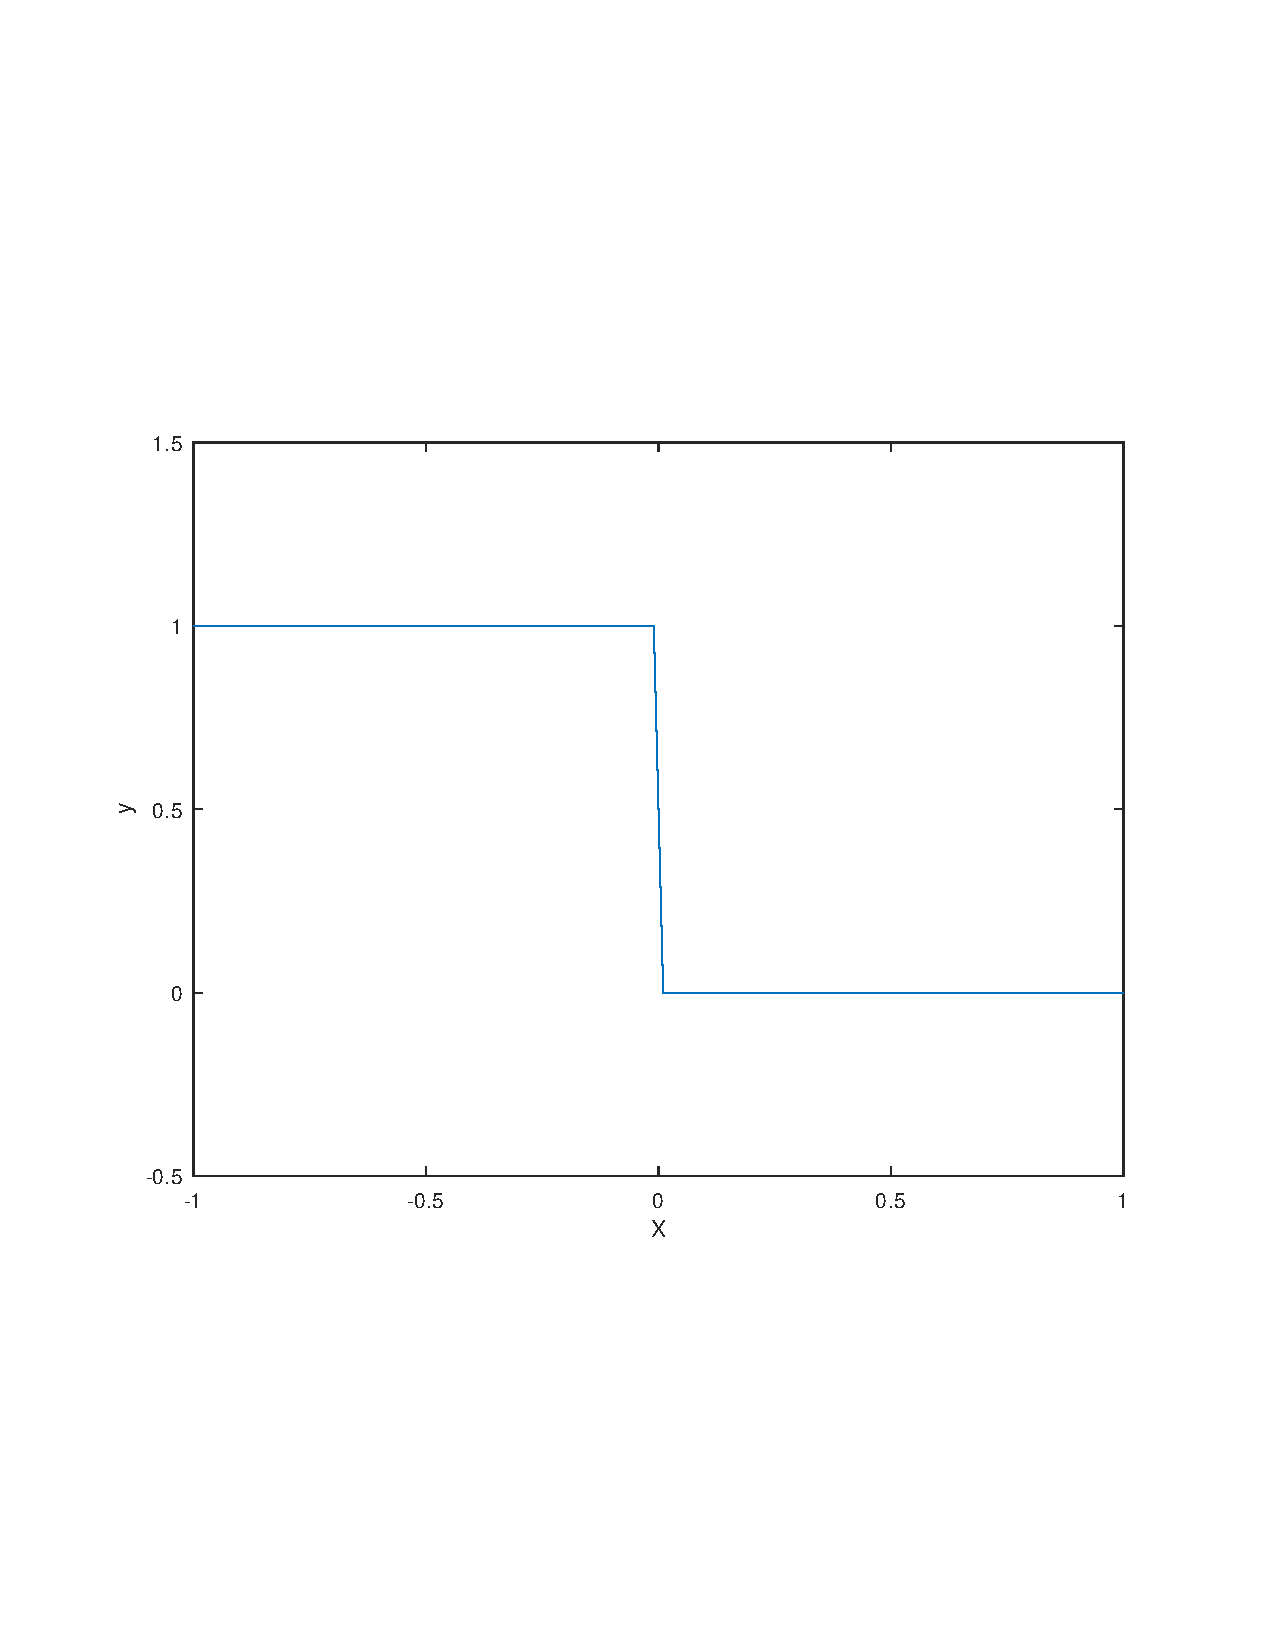
\includegraphics[width=\textwidth]{07-Graficos/partida.pdf}

    \column{0.5\textwidth}
      \begin{codeblock}
	\verbatiminput{CODEXAMPLES/plot_example.m}
      \end{codeblock}



  \end{columns}

\end{frame}

\mode<all>

\section{Bibliografía}
\mode<article>
Este material sirve simplemente como guía, pero usted puede tomar las ideas principales
y buscar bibliografía extra. A continuación puede encontrar algunos libros que pueden
servir como consulta más general.

\begin{figure}
  \includeslide[width=\textwidth]{FrameBibliografia}
\end{figure}

\mode*
\begin{frame}<presentation>[label=FrameBibliografia]
  \frametitle{Bibliografía}

  \begin{itemize}

    \item Jaan Kiusalaas, Numerical Methods in Engineering with Matlab.

    \item García de Jalón y Rodríguez, Aprenda Matlab 7.0 como si estuviera en primero.

    \item  Stephen Chapra, Numerical Methods for Engineers.

  \end{itemize}

\end{frame}

\mode<all>

\end{document}
